L'étude du cas des quadrilatères a montré que la convexité était un ingrédient central. Ceci sera aussi le cas pour les \ngones, bien que moins immédiat à justifier, comme nous le verrons dans le fait \ref{max-is-conv}, dont la preuve est indépendante des résultats de cette section.
%
Ceci explique que nous allons chercher à justifier l'existence d'au moins un \ngone\ convexe d'aire maximale parmi les \ngones\ convexes de longueur fixée. Nous allons presque y arriver...


% ----------------------- %


\begin{fact} \label{conv-pos-det}
    Si $\setproba{P} = A_1 A_2 \cdots A_n$ est un \ngone\ convexe, alors nous avons l'une des deux alternatives suivantes.
    %
	\begin{itemize}
		\item $\forall (i, k) \in \ZintervalC{1}{n}^2$,
		$\det \big( \vect{A^{\,\prime}_i A^{\,\prime}_{i+1}}, \vect{A^{\,\prime}_i A^{\,\prime}_k} \big) \geq 0$.

		\item $\forall (i, k) \in \ZintervalC{1}{n}^2$,
		$\det \big( \vect{A^{\,\prime}_i A^{\,\prime}_{i+1}}, \vect{A^{\,\prime}_i A^{\,\prime}_k} \big) \leq 0$.
    \end{itemize}
\end{fact}


\begin{proof}
    Le cas $n = 3$ étant immédiat, nous allons supposer $n \geq 4$. 
    %
    Comme $\setproba{P}$ est un \ngone, nous savons que ses sommets sont distincts deux à deux, et qu'aucun triplet de sommets consécutifs alignés n'existe. 
    %
    Dès lors, dans le plan orienté, les trois premiers sommets sont placés suivant l'une des deux configurations suivantes. 
    
    \begin{multicols}{2}
    	\small\itshape\centering
    	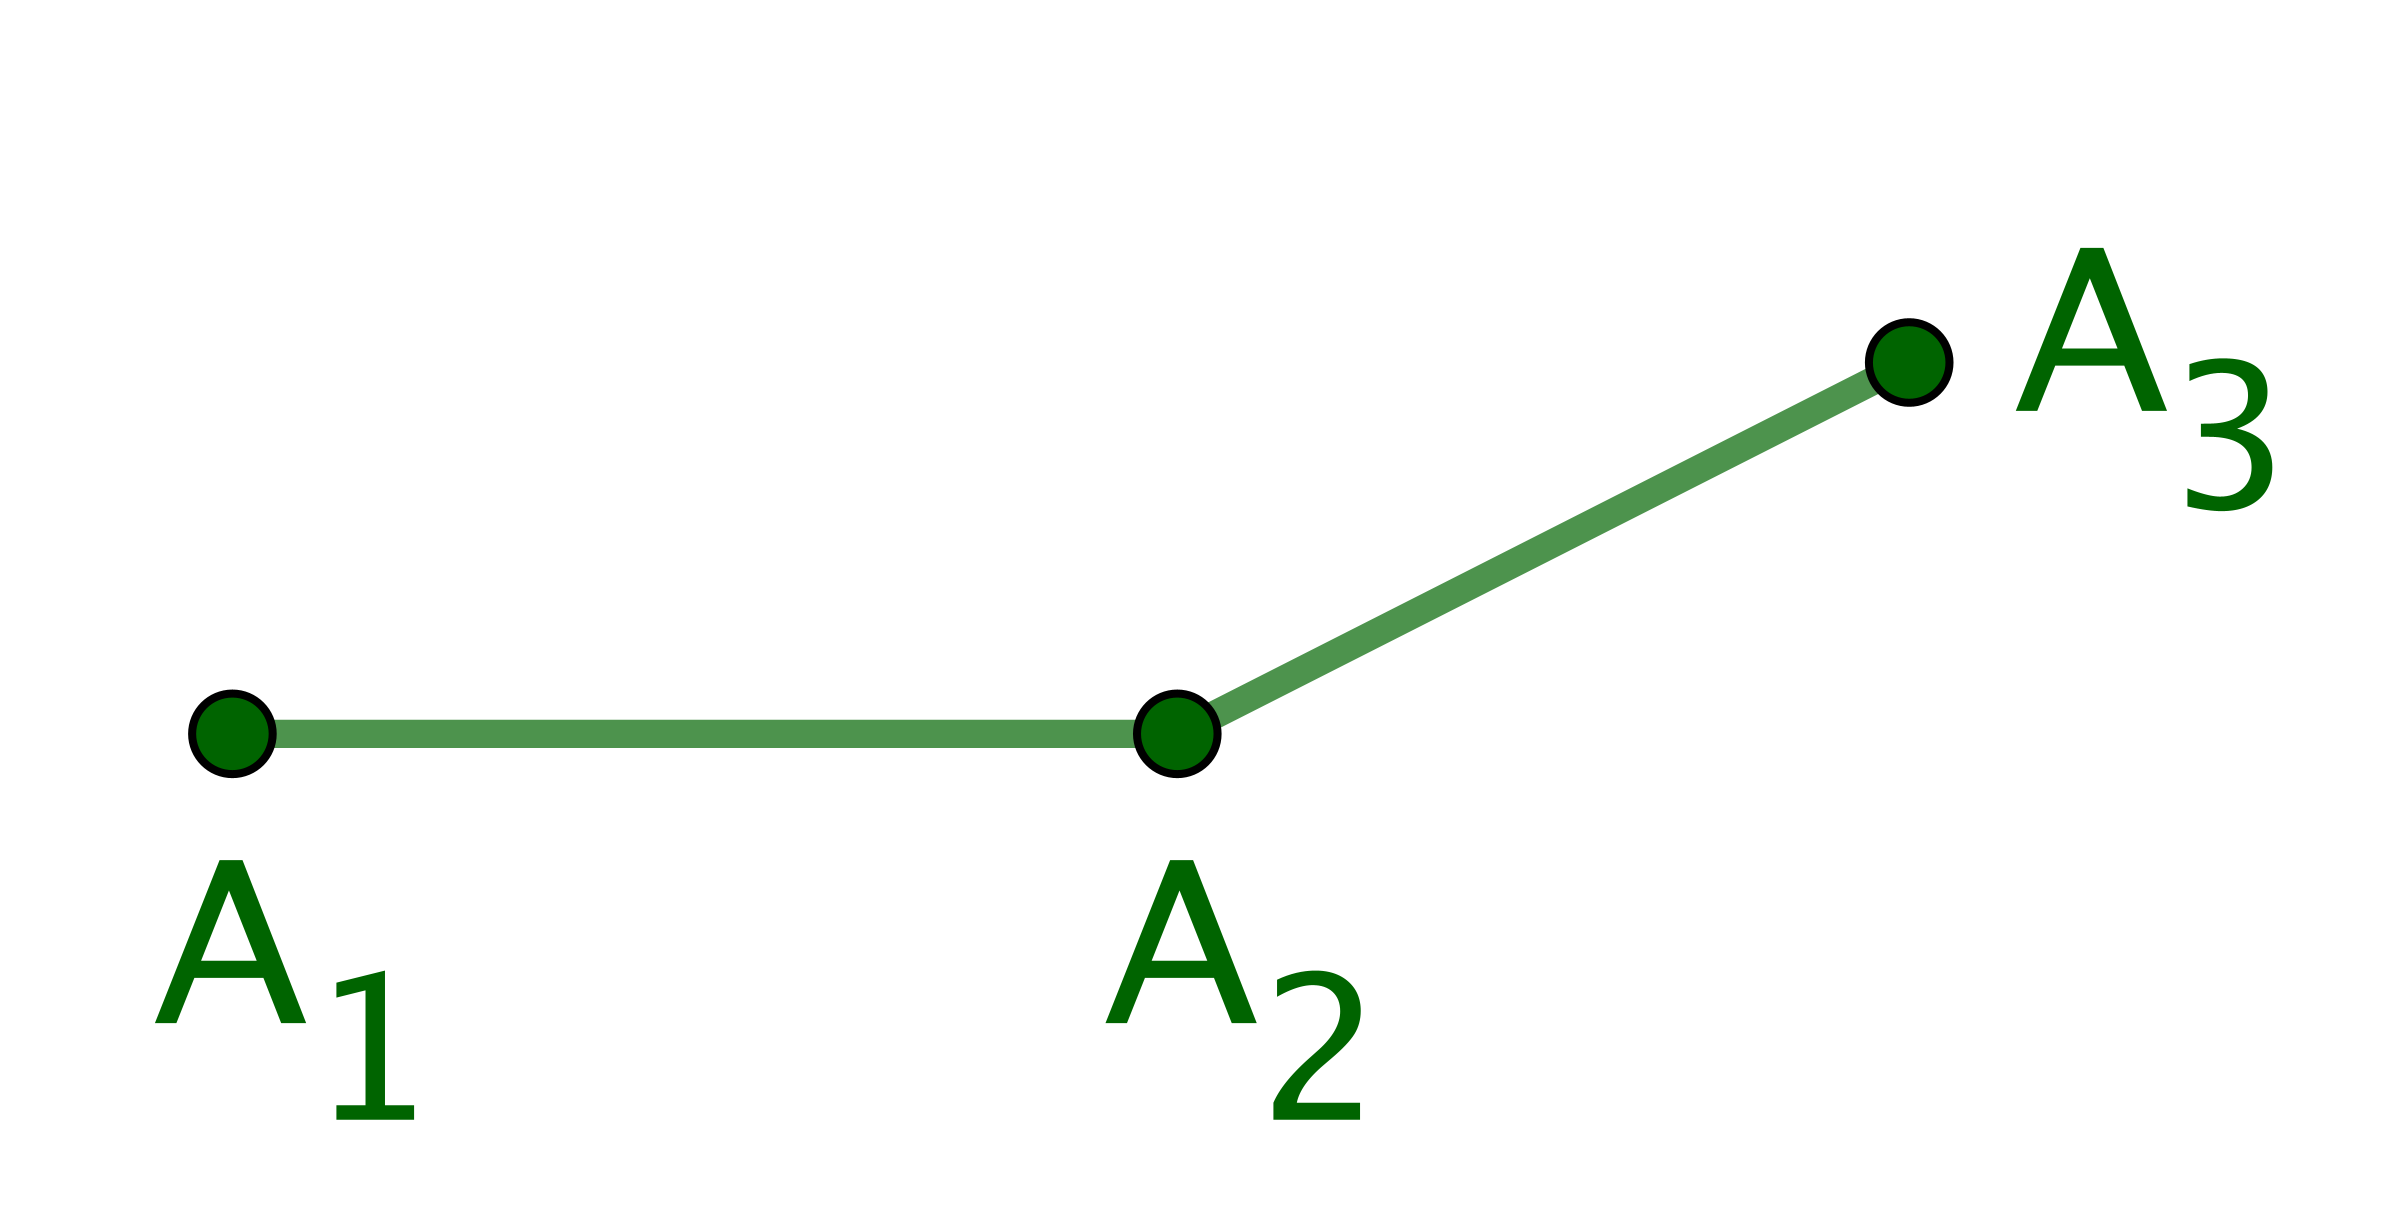
\includegraphics[scale=.45]{content/polygon/at-least-one/conv-det-sign-1.png}
	    
	    \smallskip
	    Cas positif.
    
    	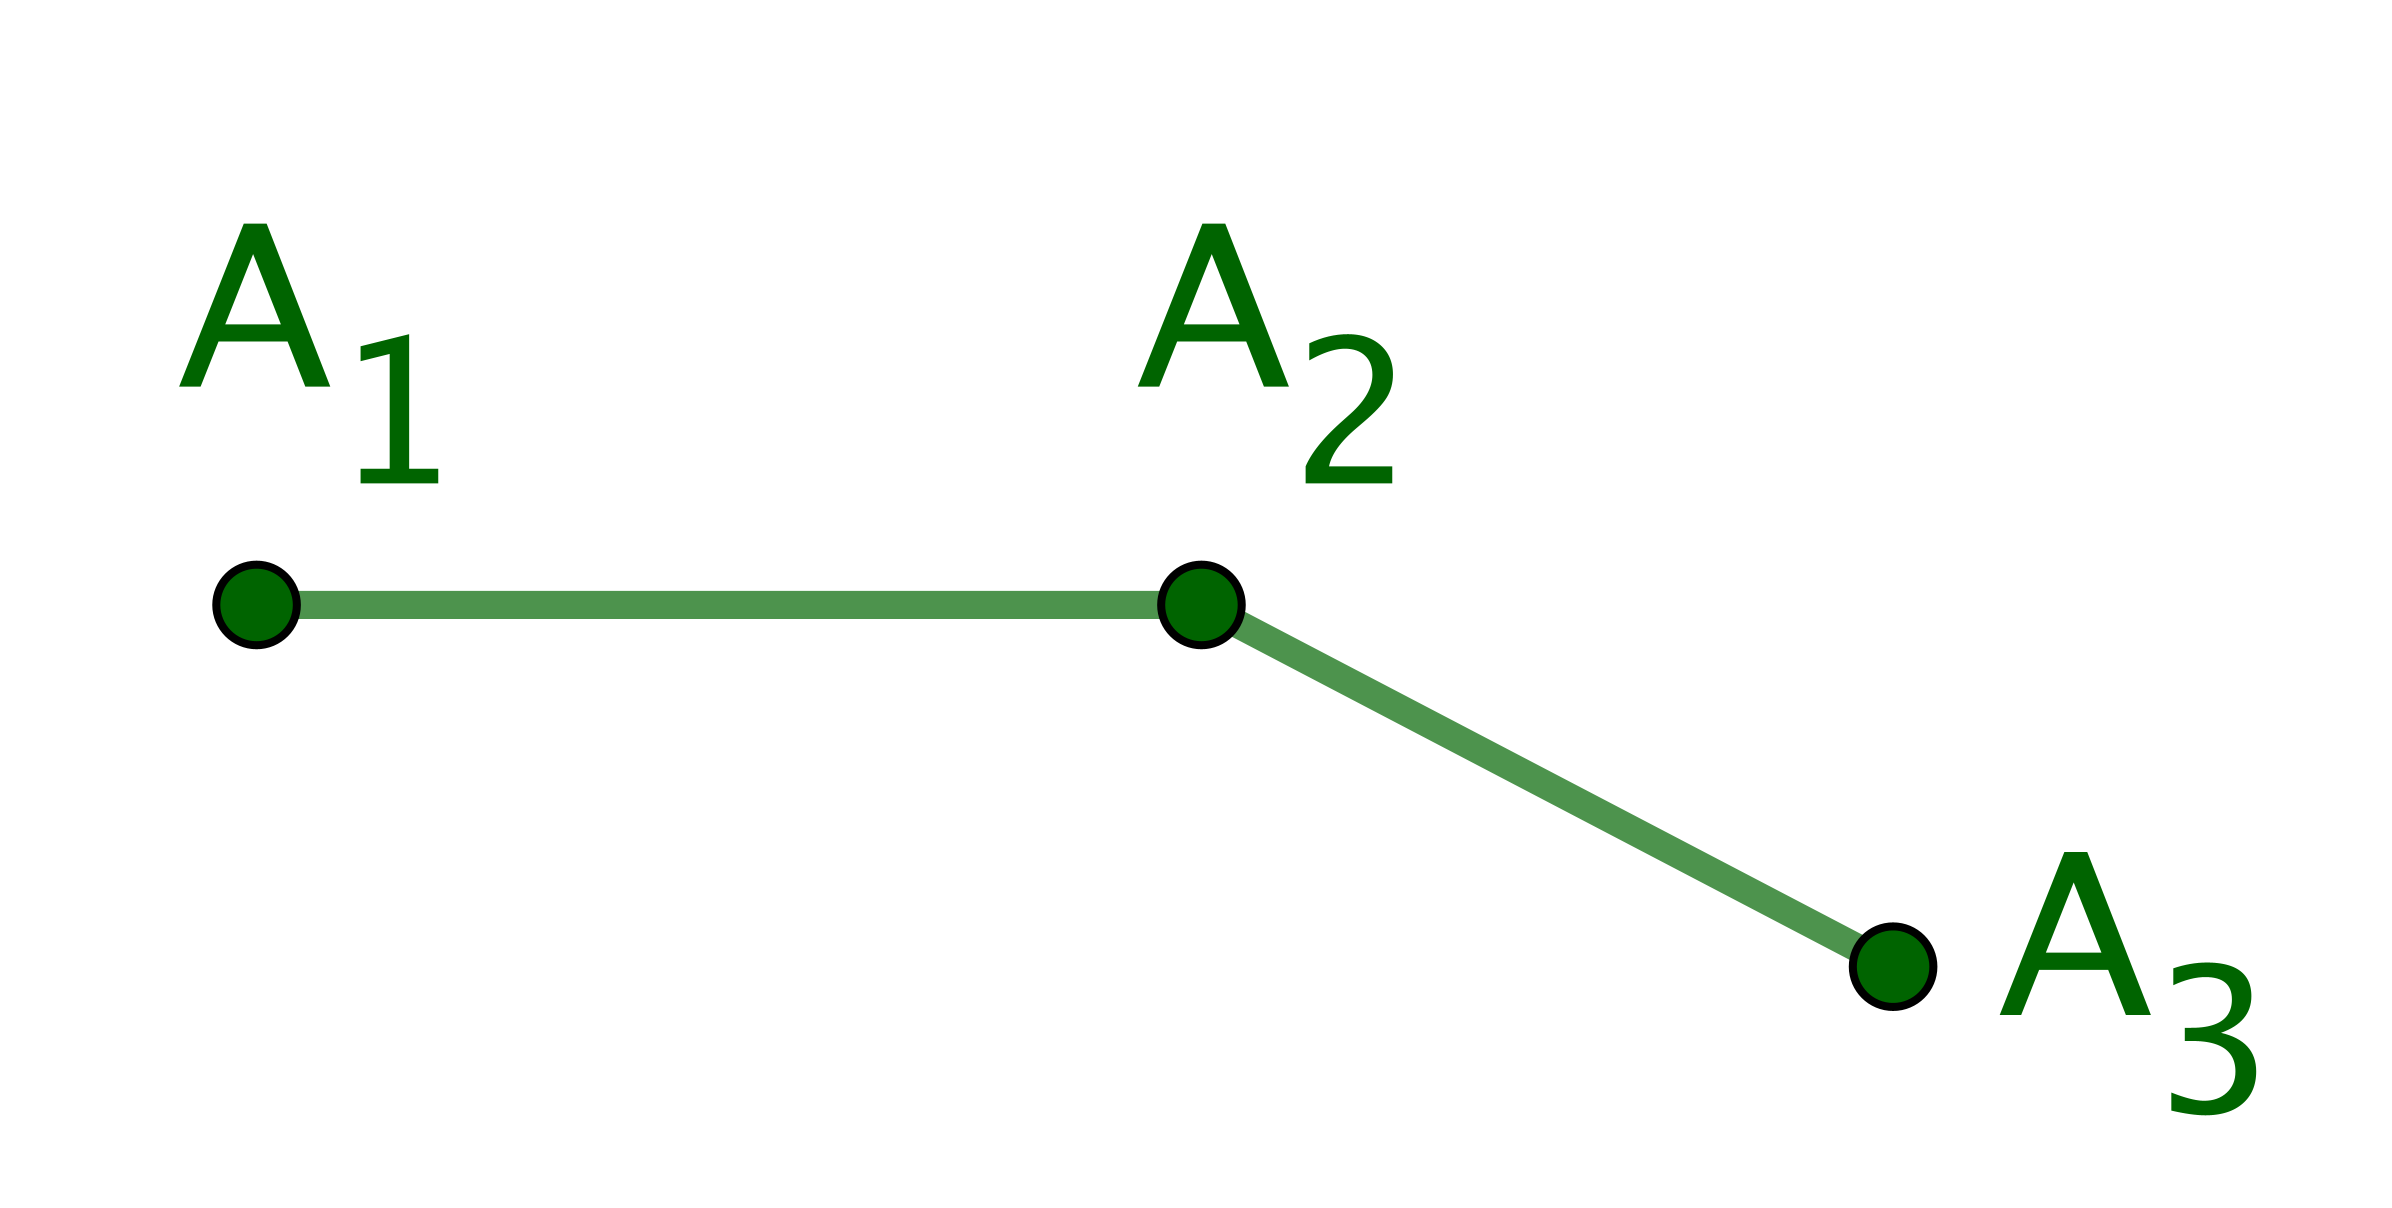
\includegraphics[scale=.45]{content/polygon/at-least-one/conv-det-sign-2.png}
	    
	    \smallskip
	    Cas négatif.
    \end{multicols}

    
    \newpage
    
    Considérons le cas positif, c'est-à-dire supposons que 
    $\det \big( \vect{A^{\,\prime}_1 A^{\,\prime}_2}, \vect{A^{\,\prime}_1 A^{\,\prime}_3} \big) > 0$.
    %
	\begin{itemize}
		\item $\vect{A^{\,\prime}_1 A^{\,\prime}_3} = \vect{A^{\,\prime}_1 A^{\,\prime}_2} + \vect{A^{\,\prime}_2 A^{\,\prime}_3}$
		donne
		$\det \big( \vect{A^{\,\prime}_2 A^{\,\prime}_3}, \vect{A^{\,\prime}_2 A^{\,\prime}_1} \big) > 0$.


		\item Comme $A_2$, $A_3$ et $A_4$ ne sont pas alignés, et de plus $A_1$ et $A_4$ du même côté de la droite $(A_2 A_3)$, nous obtenons
		$\det \big( \vect{A^{\,\prime}_2 A^{\,\prime}_3}, \vect{A^{\,\prime}_2 A^{\,\prime}_4} \big) > 0$.


		\item En continuant de proche en proche, nous arrivons à
		$\det \big( \vect{A^{\,\prime}_i A^{\,\prime}_{i+1}}, \vect{A^{\,\prime}_i A^{\,\prime}_{i+2}} \big) > 0$
		pour $i \in \ZintervalC{1}{n}$ quelconque.


		\item Le point précédent et la convexité donnent
		$\det \big( \vect{A^{\,\prime}_i A^{\,\prime}_{i+1}}, \vect{A^{\,\prime}_i A^{\,\prime}_k} \big) \geq 0$
		pour $(i, k) \in \ZintervalC{1}{n}^2$ tel que $k \notin \setgene{i ; i+1}$.
    \end{itemize}

    \smallskip
    
    Le cas négatif se traite de façon similaire. 
\end{proof}


% ----------------------- %


On aurait pu établir des inégalités strictes pour les indices $k \notin \setgene{i ; i+1}$, mais nous n'aurons pas besoin de cette précision, car nous allons travailler dans un ensemble compact, et donc fermé, de \ncycles.
Ceci aura pour inconvénient de ne pas garantir le caractère $n$-gonal, mais nous n'avons pas le choix!


\begin{fact} \label{at-least-one-ncycle}
    Soient $n \in \NN_{\geq3}$,
    $\ell \in \RRsp$,
    $\pvaxes{O | i | j}$ un repère orthonormé direct du plan
    et
    $\setproba{U} \subset \RR^{2n}$ l'ensemble des uplets de coordonnées $\big( x(A_1) ; y(A_1) ; \dots ; x(A_n) ; y(A_n) \big)$ où $\setproba{L} = A_1 A_2 \cdots A_n$ désigne un \ncycle\ vérifiant les conditions suivantes.
    %
    \begin{itemize}
        \item $\cyclelen{\setproba{L}} = \ell$.
    
        \item  $\forall (i, k) \in \ZintervalC{1}{n}^2$,
		$\det \big( \vect{A^{\,\prime}_i A^{\,\prime}_{i+1}}, \vect{A^{\,\prime}_i A^{\,\prime}_k} \big) \geq 0$.
    \end{itemize}
    
    On considère alors la fonction $\alpha: \setproba{U} \rightarrow \RRp$ qui à un uplet de $\setproba{U}$ associe l'aire algébrique du \ncycle\ qu'il représente.
   	%
	Avec ces notations, la fonction $\alpha: \setproba{U} \rightarrow \RRp$ admet au moins un maximum.
\end{fact}


\begin{proof}
     $\setproba{U}$ est fermé dans $\RR^{2n}$, car les conditions le définissant le sont, et il est borné, car inclus dans la boule fermée de centre $\pt{O}$ et de rayon $\ell$,
     donc $\setproba{U}$ est un compact de $\RR^{2n}$.
     De plus, $\alpha$ est continue d'après le fait \ref{sarea-cont}.
     Finalement, par continuité et compacité, $\alpha$ admet un maximum sur $\setproba{U}$.
\end{proof}


% ----------------------- %


Nous arrivons, ci-dessous, au résultat central pour les \ngones\ convexes où la perte éventuelle de sommets est un faux problème, car nous aboutirons, plus tard, à la comparaison de \kregs\ convexes pour $k$ variable, une tâche aisée, puisque le périmètre et l'aire d'un \kreg\ convexe s'expriment en fonction de $k$.


\begin{fact} \label{at-least-one-kgone}
    Soient $n \in \NN_{\geq3}$ et $\ell \in \RRsp$.
    Il existe un \kgone\ convexe $\setproba{K}$ validant les assertions suivantes.
    %
	\begin{itemize}
		\item $k \leq n$ et $\cyclelen{\setproba{K}} = \ell$.

		\item Si $\setproba{P}$ est un \ngone\ convexe tel que $\cyclelen{\setproba{P}} = \ell$, alors $\area{\setproba{P}} \leq \area{\setproba{K}}$.
    \end{itemize}
\end{fact}


\begin{proof}
	Commençons par chercher un \ncycle\ $\setproba{M}$ tel que $\area{\setproba{P}} \leq \area{\setproba{M}}$ pour tout \ngone\ convexe $\setproba{P}$ vérifiant $\cyclelen{\setproba{P}} = \ell$.
	%
	\begin{itemize}
		\item 
    \end{itemize}
    
    
	
	XXXX
	
	
	Commençons par noter que tout \ncycle\ d'origine $A_1$ translaté via le vecteur $\vect{A_1 \pt{O}}$ donne un \ncycle\ d'origine $\pt{O}$, sans modification de la longueur, ni de l'aire algébrique, ni l'ordre des sommets après $A_1$.
    %
    De plus, selon le fait \ref{conv-pos-det},
    $\sarea{\setproba{L}^{\mathrm{op}}} = - \sarea{\setproba{L}}$ pour tout \ncycle\ $\setproba{L}$ d'après le fait \ref{nline-rota-opp}, donc nous pouvons nous concentrer sur les \ncycles\ convexes vérifiant $\det \big( \vect{A^{\,\prime}_i A^{\,\prime}_{i+1}}, \vect{A^{\,\prime}_i A^{\,\prime}_k} \big) \geq 0$ pour tous les sommets $A_i$ et $A_k$ grâce au fait précédent.


	\begin{itemize}
		\item Munissons le plan d'un repère orthonormé direct $\pvaxes{O | i | j}$, puis notons $\setproba{U} \subset \RR^{2n}$ l'ensemble des uplets de coordonnées $\big( x(A_1) ; y(A_1) ; \dots ; x(A_n) ; y(A_n) \big)$ où $\setproba{L} = A_1 A_2 \cdots A_n$ est un \ncycle\ vérifiant les conditions suivantes.
	    %
	    \begin{enumerate}
	    	\item $A_1 = \pt{O}$.

	    	\item $\cyclelen{\setproba{L}} = \ell$.

		    \item
		    $\forall (k, i) \in \ZintervalC{1}{n}^2$,
		    $\det \big( \vect{A^{\,\prime}_i A^{\,\prime}_{i+1}}, \vect{A^{\,\prime}_i A^{\,\prime}_k} \big) \geq 0$.
	    \end{enumerate}


        \item $\setproba{U}$ est fermé dans $\RR^{2n}$, car les conditions le définissant le sont, et il est borné, car inclus dans la boule fermée de centre $\pt{O}$ et de rayon $\ell$.
        En résumé, $\setproba{U}$ est un compact de $\RR^{2n}$.


        \item Nous définissons la fonction $\alpha: \setproba{U} \rightarrow \RRp$ qui à un uplet de $\setproba{U}$ associe l'aire algébrique du \ncycle\ qu'il représente.
        Cette fonction est continue d'après le fait \ref{sarea-cont}.
        %
        Donc, $\alpha$ admet un maximum sur $\setproba{U}$ par continuité et compacité. Affaire conclue!
        
        
        \item Reprenons les notations de la preuve du fait \ref{at-least-one-ncycle}, puis notons $\setproba{K}$ un \ncycle\ convexe maximisant la fonction $\alpha$ sur $\setproba{U}$, de sorte que $\cyclelen{\setproba{K}} = \ell$ est validée.
		%
		Il est immédiat que pour tout \ngone\ convexe $\setproba{P}$ tel que $\cyclelen{\setproba{P}} = \ell$, nous avons $\sarea{\setproba{P}} \leq \sarea{\setproba{K}}$, puis le fait \ref{sarea-ngone} donne que $\area{\setproba{P}} \leq \abs{\sarea{\setproba{K}}}$, après avoir noté que nécessairement $\sarea{\setproba{K}} \geq 0$.
		%
		Pour finir, voyons pourquoi $\setproba{K}$ est un \kgone\ convexe avec $k \leq n$, ce qui impliquera ensuite $\abs{\sarea{\setproba{K}}} = \area{\setproba{K}}$.
    \end{itemize}
	
	\null\vspace{-6ex}
\end{proof}

Affaire conclue!
